\documentclass[11pt]{article}

\newcommand{\define}[2] {
  \textbf{Definition: #1}
  \begin{center} #2
\end{center}
}

\usepackage{graphicx}


\begin{document}

\title{Extreme computing: Assignment 1 \\ S0936300}
\maketitle

\section{Introduction}

This following is a report on suggestions with a proposed solution for Massbase's recommender systems with the aim of being able to recommend products based on a users facebook or twitter updates(known as blips).

There is some gaps in the information given. We do not know how many users will be using the system and as it is a start-up company it seems feasible that in the first year the user base may not be high, but will increase more rapidly as time progresses. Thus,a solution that allows for easy extension is ideal, allowing for less of the budget to be used in the first year and more for the second as the user-base grows. If the user-base does not grow as expected in the first year, the spare money could instead be spent directly on addressing this using advertising other other methods.

\section{Design considerations and alternatives}

For this project there are a large amount of design considerations.

\begin{enumerate}
\item How are we going to obtain the BLIP data?
\item How are we going to obtain product data to actually recommend?
\item How are we going to get initial data on the user? We can't start recommending on the day if we know little about them.
\item Parallel database systems vs Hadoop
\item Real time vs later recommendations
\end{enumerate}

BLIPS will be received with the following information

\begin{itemize}
\item Unique id
\item Time/data
\item User
\item Blip text
\item explicit tags(location, time, hashtags, other users)
\end{itemize}

In addition to explicit tags, post-processing and natural language processing is required to obtain implicit tags such as movie names, events, other user's identified in the blip. 

The following explicit tags are used for consideration:

\begin{itemize}
\item Movie
\item Product
\item Event
\item User (if it is an associated user)
\end{itemize}

Later the system could be extended to deal with locations(give recommendations of interesting areas a user may like), or food/restaurants in an area.

\subsection{Propriety data collection}

\subsubsection{Initial user data collection}
One of the problems discussed in the 'Design considerations' section is obtaining initial user data. If the user signs up, how would we be able to offer recommendations on the day if we have no data on them? 

One approach would be to use an initial questionnaire to snapshot a users likes and interests and as blips are acquired update and adjust accordingly. As a further source of information, facebook's api provides a vast amount of data on users such as movie/tv show likes, events attended, interests, age range(possibly useful for post-processing), locations visited and references to other users(creating an initial view of the users social network). A disadvantage of this in comparison to a questionnaire is that 'likes' happen over a long period of time, may not be removed or updated and consequently may not be an accurate representation of a person(for example as one moves from teens to adult their taste in genre of film may change, but this may not be obvious in facebook's data). 

\subsubsection{Initial data collection of recommendations}
Before we can start recommending movies, tv shows, events or products we first need to acquire data on what is already available. Firstly we could scrap information from various sites however this could be too time consuming and for some websites this is against their TOS. Fortunately, API's exist for a large portion of information that we need.

Amazon and Ebay both provide api's for accessing their product information. Furthermore, Amazon offers easy searching of similar products, we could use to cross reference with our user information to provide more accurate recommendations than Amazon themselves. In addition, Massbase can obtain referral fees for products brought on amazon, providing another method of monetising the idea and not simply depending on subscriptions. One of the limitations of using amazon's api is that it is restricted to 3,600 api calls an hour and if we choose to send bulk recommendation emails to everyone instead of doing this in real time, this could be exceeded within the hour. Api calls are increased if more than 4600\$ph worth of products are purchased through us, but as massbase is just starting out this may not be feasible and we are thus assuming ourselves to be restricted to 3,600.

In addition, Movie and TV show data can be obtained using API's provided by 'Rotten Tomatoes', providing a database of movies/tv shows available, genres and crowd sourced movie ratings. Further, the api will grant us a list of new films in cinema and new dvd's being released. An alternative to 'Rotten tomatoes' is 'MyMovie api' which instead takes information from IMDB. The limitations of both 'IMDB' and 'Rotten Tomatoes' is an allowance of only 10,000 and 2,5000 api calls per day and the user-base expected will be too large. Licences can be obtained to increase this although no information on prices could be found.


\subsection{Getting blips}

There are a variety of considerations for acquiring blip information. Firstly, we could periodically poll facebook/twitter/other sources servers, detect changes and update. This seems a less efficient method of doing so however if the server-load is extremely heavy, we could slightly delay the time we do this, allowing the server to reduce it's load and then continue and we would not need to worry about caching incoming data when the server load is high. Duplicate removal would also requires some thought, if we're periodically polling for information it's likely we will obtain duplicate blips often and as such duplication should be run after each poll.

Fortunately there is an alternative to the above. Facebook and twitter's API's allow for notifications of updates so we do not need to continuously poll their servers and need only to cache the data and changes. We can then check for duplicate information on arrival and ignore the blip if it already exists. Further, if a user updates their facebook status and a twitter update comes within minutes there is a higher probability that they are duplicates and this assumption may be used to further quicken the process.

One problem to highlight with the whole project proposition is the feasibility of acquiring blips from facebook/twitter updates. How often do users post status updates about the products they have purchased or the films that they watched unless they were really, really good? And even so, this doesn't seem to be even a weekly occurrence. Posting about event attendance and friends who were in attendance seems more common especially in the younger age ranges. Thus, facebook and twitter may be a good source for identifying social networks and events attended but not for acquiring information on products or movies watched. 

As a method to compensate, netflix was looked upon however this cannot be used as their api is no longer available for public access. 

\subsection{Real time recommendations vs batch}
From a user perspective, real-time recommendations do not seem like a good option. If for every facebook/twitter update we receive an email recommending products(which we frequently get emails about anyway) it could get quite annoying. An overnight email is therefore preferred but this creates a greater challenge. If we run the recommendation system at a set time for all users we are likely to exhaust the amount of available api calls per hour.

\subsection{Database considerations}
Parallel databases are very trailed and proven approach that is effective and efficient. Hadoop however is recommended for large scale data analysis and as such would be ideal when used for when applying recommendations themselves. We could use parallel databases for this, but the speed and ability of hadoop means we are not limited to the amount of input so if users stay with the system over a period of years we wont be required to prune data and can even observe how their tastes change over a period of time. Hadoop also naturally sorts based on keys.

With looking at the problem are three possible databases that may be required depending on the chosen approach:

\begin{itemize}
\item A database of recommendations
\item tags database (tag, user, location, time, tag properties)
\item BLIP Cache/store.
\end{itemize}

When considering temporal locality we could have a separate database for more recent blips but this is not required if blips are in the database by the order of their time stamp. There is a requirement to be able to group tags by location, or locations by tags. This would be relatively easy with the above tag database. 

\section{Proposed solution}
It is suggested that the company does not build a system from scratch and instead uses available services/clouds. If later the user-base extends and more funding is given, the system could be transferred to a custom built cloud. 

\subsection{Propriety work: Data collection}
Before the design of the system can be started, propriety data collection is required. For product recommendations, Amazon provide all information in a very accessible format and 3,600 api calls should be enough especially if users are in different time zones and thus require emails at different times. This would allow us to batch recommendation processing into different hours as more calls become available. Further as the amount of users and products purchases increase, the api calls available increase, allowing flexibility without further costs.

To obtain a database of initial products and services to recommend in the movie/tvshows area it is suggested that over a period of a few days we take information from IMDB/Rotten tomatoes such as names, ratings, and genres and store this is a database which could be very quickly accessed. This reduce the impact of the limit we are required to work within. As new information becomes available we can update the database or use the 10,000 api calls to go over data in the database and make sure there have been no vast changes (in ratings for example). A simple parallel database if suggested to be used for storing recommendation data, Hadoop is mostly used when Petabytes of data are required to be stored and analysed and it is not presumed that this will required.

Using facebook and twitters api we can obtain blips at run-time instead of polling their servers and store this in a cache. We can remove duplicates at runtime by checking if they are already in the database and ignore them if they are, reducing later processing needs.

MapReduce provides an appropriate paradigm to use given the large amount of data that needs to be required and the opportunity to work in batch. It is also easy to extend by adding more mappers and reduces as the amount of data increases. A final advantage of Hadoop is automatically sorting keys, each mapper receives unique users information so users are not split between mappers so that each reducer outputs complete information about a list of users. The recommender database is a parallel-base to allow for speed and efficiency, there was no forseen reason for using map reduce.

\subsection{System design}

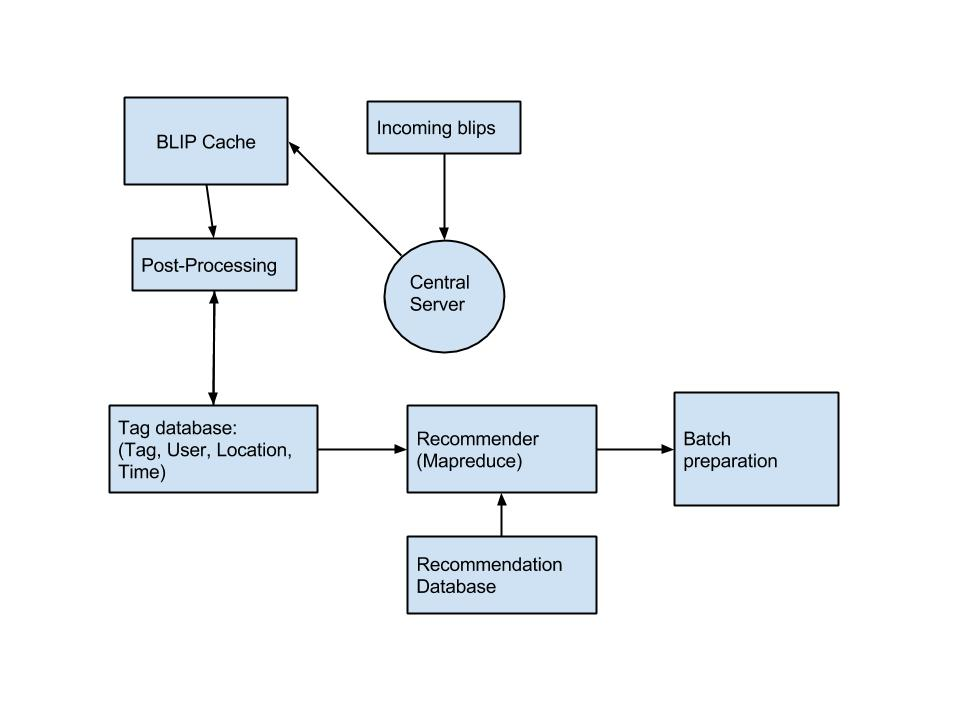
\includegraphics[scale=0.4]{database}

The diagram above is the proposed solution. Firstly blips are sent to the central server where duplicates are checked. If no duplicates are found they are forwarded to the BLIP cache. The central server is also responsible for initialising the recommender and sending emails. The 'Post-processing' then takes blips from the cache, finds any implicit or explicit tags and forwards these to the tag database. Post-processing can also look up in the "Recommend database" to add additional information to tags such as genres or ratings of films so we do not need to do this on the fly next time or every time a recommendation is required. The recommender database has a list of products, their types and other properties that can be accessed and sorted quickly.

In the tag database, each row has information on:

\begin{itemize}
\item Tag
\item User associated with tag
\item location the tag/blip occured
\item time the tag was created
\item tag type
\item tag properties: genres, ratings, categories, etc.
\end{itemize}

Tags are stored individually so if there are multiple tags in a blip, multiple tags will be sent to the database. The benefit of this is that is allows us to sort information on one attribute easily and thus sort on location, user, associated users, tag types, time, etc. Furthermore, the lower the tag in the database, the more recent it is which allows us to consider temporarily when recommending(we can always just feed the last x amount of tags for a user). 

The tag database is then input into the recommender which uses Map-reduce. The mapper sorts blips into (key, values) where key is the username and the value is the rest of the blip from the tag database. The reducer then condenses this into (user, (tag, tag-type, properties)...) for example ("Ben", ("War of the worlds", Movie, Thriller), ("Helen", friend)).

Recommendations can then be made in parallel by sorting through the output from the reducer. It can easily take out tags of a specific type, search the recommendations database for a list of items with the same type and apply a chosen algorithm.

\begin{thebibliography}{9}

\bibitem{tradeoff}
Tradeoffs between parallel database systems, hadoop, and hadoopdb as platforms for petabyte-scale analysys. Daniel J. Abadi

\end{thebibliography}

\end{document}

